%====================================================================================
\section{Prueba de hipótesis sobre un solo parámetro de población: la prueba t}
%====================================================================================

%------------------------------------------------------------------------------------
\subsection{t-student}
%------------------------------------------------------------------------------------

\begin{frame}{Inferencia 1: prueba de hipótesis para una única combinación lineal de coeficientes}
	Consideremos nuevamente el siguiente modelo (o PGD) con una constante y más de un regresor
		$$Y_i = \beta_0 + \beta_1 X_{1i} + \beta_2X_{2i} + u_i$$
	La inferencia es el proceso de realizar una prueba estadística; nos interesa la importancia de los efectos sobre la variable dependiente. En particular, el coeficiente de interés es el efecto de $X_2$ sobre $Y$. El efecto de $X_1$ e $Y$ es necesario porque eso nos permite controlar otros efectos. Por ejemplo
		\begin{align*}
			H_0 & : \beta_2 = 0\\
			H_a & : \beta_2 \neq 0
		\end{align*}
	por tanto, podemos centrarnos sólo en algún parámetro de interés, en este caso $\beta_2$. \textit{[Pregunta: ¿Por qué deberíamos mantener en el análisis la variable $X_1$?. Son controles]}.
\end{frame}
%---------------------------------------------------
\begin{frame}{Antes de la inferencia}
	Cuando configuramos un modelo, tenemos los siguientes tipos de regresores:
		\begin{itemize}
			\item Regresores o variables de interés (relacionadas con la política).
			\item Variables de control.
		\end{itemize}
	Si alguna variable no se puede clasificar en las categorías anteriores, no la considere en su análisis.
\end{frame}
%---------------------------------------------------
\begin{frame}{¿Z o t-student?}
	Ya hemos discutido este tema con respecto a Z o t-student. Básicamente, debemos elegir la estadística según el número de observaciones bajo análisis. Una regla simple es: una muestra pequeña tiene menos de 150 observaciones; en ese caso nuestro análisis considera el t-student. La estadística es:
		$$t_{cal} = \frac{\textup{Estimador - Prueba de hipotesis}}{\textup{Error estandar del estimador}}$$
	por ejemplo.
		$$t_{cal}=\frac{\widehat{\beta}_2 - 0}{S.E(\widehat{\beta}_2)}$$
	luego contrastamos esa $t$ \textit{"realmente calculada"} con valores críticos o simplemente calculamos el \textit{p-value} asociado a esa prueba; es decir, $2Pr(t > |t_{cal}|)$
\end{frame}
%---------------------------------------------------
\begin{frame}{t-student}
	\begin{itemize}
		\item Aunque el $\widehat{\beta}_{j}$ teóricamente sigue una distribución normal, al depender de $\sigma^2$ (parámetro no conocido) hace que el uso del estimador $\widehat{\sigma}^2=SRC/(n-k-1)$ cambie la distribución del parámetro.
		\item Conociendo la distribución se pueden probar diversas hipótesis como $H_{0}:\beta_{j}=0$ en cuyo caso, si se prueba esa hipótesis la variable $x_{j}$ no tiene efecto sobre $y$ controlando por las otras $x's$
		\item El $t$ estadístico para dicha hipótesis sería $t_{\beta_{j}}\equiv \frac{\widehat{\beta}_{j}-0}{Se(\widehat{\beta_{j})}}$ que sigue una distribución T de student con $n-k-1$ grados de libertad.
		\item Aunque con muestras grandes la T de student se comporta como una normal. Específicamente cuando $n-k-1>120$ se puede usar una normal para los valores críticos.
	\end{itemize}
\end{frame}
%---------------------------------------------------
\begin{frame}{t-student}
	\begin{itemize}
		\item Además de la hipótesis nula $(H_{0})$ para completar la prueba estadística se necesita de una hipótesis alternativa $(H_{1})$ y de un nivel de significancia.
		\item $H_{1}$ puede ser de unilateral o de un lado o bilateral o de dos lados
		\item Unilateral:$\beta_{j}>0$ o  $\beta_{j}<0$
		\item Bilateral:$\beta_{j} \neq 0$
		\item El nivel de significancia es la probabilidad de cometer un error de tipo I, los valores frecuentemente elegidos son de 1, 5 y 10 por ciento.
	\end{itemize}
\end{frame}
%---------------------------------------------------
\begin{frame}{t-student}
	$H_{0}: \beta_{j}=0$ y $H_{1}: \beta_{j}\neq 0$ \\
	Si $t_{\beta_{j}}>|Crit|$, entonces se rechaza la hipótesis nula $H_{0}$. Donde $Crit$ se obtiene de tablas estadísticas necesitando para ello el nivel de significancia a utilizar ($\alpha$) y el número de grados de libertad $n-k-1$
	\begin{figure}[H]
		\begin{centering}
			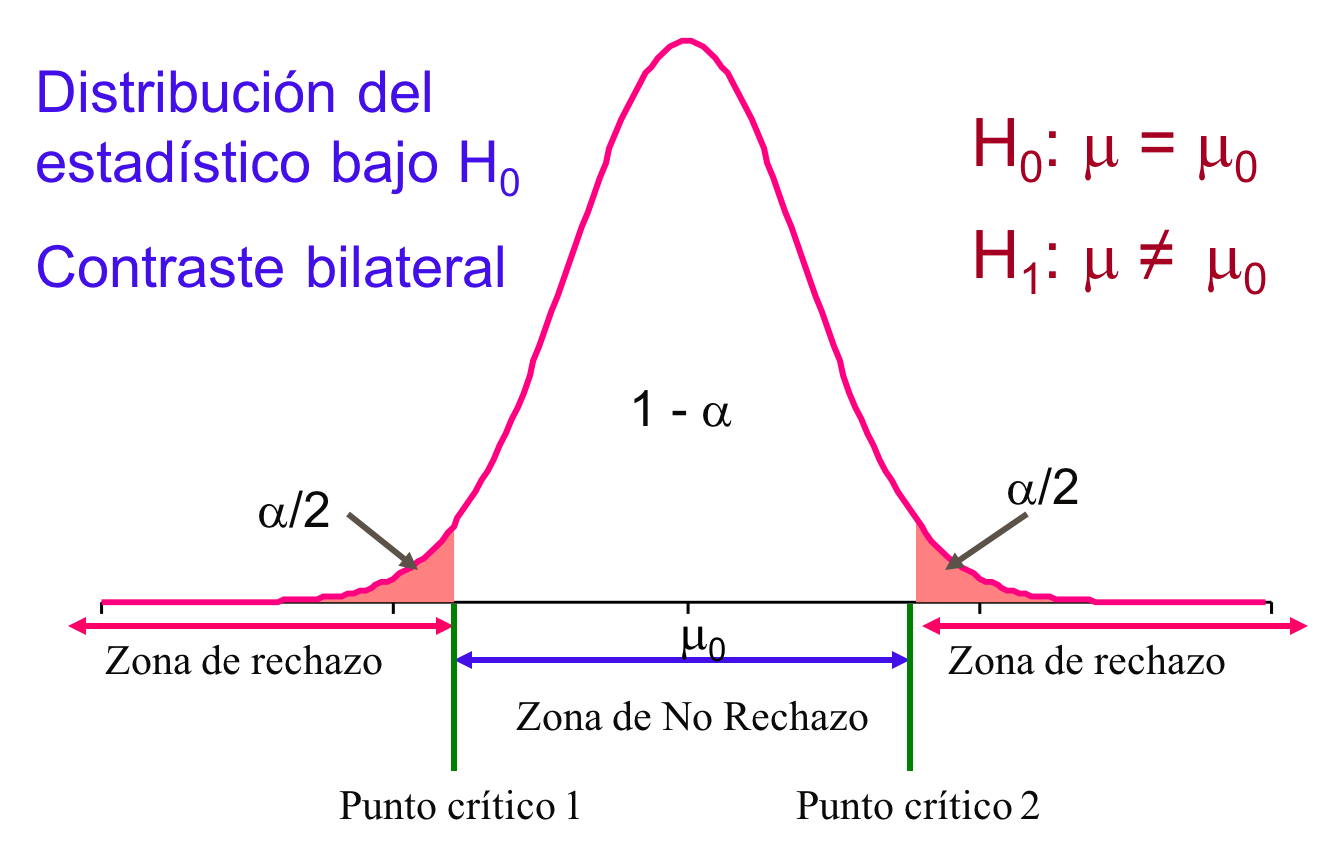
\includegraphics[scale=0.4]{fig/RegionCritica.png}
		\end{centering}
	\end{figure}
\end{frame}
%---------------------------------------------------
\begin{frame}{t-student}
	\begin{itemize}
		\item Si se rechaza la $H_{0}$ lo que típicamente se dice es que la variable $x_{j}$ es estadísticamente significativa al nivel de significancia de $\alpha$
		\item Si no se rechaza la $H_{0}$ lo que típicamente se dice es que la variable $x_{j}$ es estadísticamente no significativa al nivel de significancia de $\alpha$
		\item Aunque se vio el caso de $H_{0}: \beta_{j}=0$ en general se puede probar la hipótesis: $H_{0}: \beta_{j}=a_{j}$, en cuyo caso el t-estadístico quedaría definido por: $t=\frac{\hat{\beta_{j}}-a_{j}}{Se(\hat{\beta_{j}})}$
	\end{itemize}
\end{frame}
%---------------------------------------------------
\begin{frame}{t-student: ejemplo}
	Podemos incluir en nuestro análisis de inferencia alguna combinación lineal de parámetros. Por ejemplo, consideremos una función de producción para la economía de EE. UU.
		$$Q = e^{\alpha_0}K^{\alpha_k}L^{\alpha_l}$$
	donde $\widehat{\alpha}_k = 0.632$ y $\widehat{\alpha}_l = 0.452$. Adicionalmente, tenemos la siguiente información: $cov(\widehat{\alpha}_k, \widehat{\alpha}_l)= 0.055$, $std(\widehat{\alpha}_k)=0.257$ y $std(\widehat{\alpha}_l)=0.219$. Evaluamos is $\widehat{\alpha}_k$ son idñenticos en términos estadísticos
		$$t_{cal}= \frac{\widehat{\alpha}_k - \widehat{\alpha}_l}{S.E(\widehat{\alpha}_k - \widehat{\alpha}_l)}$$
	o si existe evidencia de retornos constantes a escala
		$$t_{cal}= \frac{\widehat{\alpha}_k + \widehat{\alpha}_l - 1}{S.E(\widehat{\alpha}_k + \widehat{\alpha}_l - 1)}$$
	luego contrastamos esa $t$ \textit{"realmente calculada"} con valores críticos o simplemente calculamos el \textit{p-value} asociado a esa prueba; es decir, $2Pr(t > |t_{cal}|)$
\end{frame}
%---------------------------------------------------
\begin{frame}{t-student: resumen de pasos}
	\begin{itemize}
		\item Calcular las estimaciones de MCO.
		\item Calcular el error estándar de las combinaciones lineales de parámetros.
		\item Calcular la estadística t-student o t "\textit{realmente calculada}".
		\item Calcular el p-value o simplemente concluya utilizando valores críticos.
		\item La interpretación es muy importante, ¡no te pierdas ese paso !.
	\end{itemize}
\end{frame}

%------------------------------------------------------------------------------------
\subsection{P-Value}
%------------------------------------------------------------------------------------
\begin{frame}{P-Value}
	\begin{itemize}
		\item Además de la prueba T y el intervalo de confianza existe un tercer enfoque para evaluar la significancia individual de los parámetros
		\item El P-value o valor P es el nivel exacto de significancia y esta definido como el nivel más bajo  de significancia al cual puede rechazarse una hipótesis nula
		\item Como regla práctica si el P-value es menor a 0.05 entonces se dice que se rechaza la nula a un nivel de significancia del 5 por ciento
		\item La ventaja del uso de este indicador es que no requiere observar ninguna tabla estadística, sólo comparar el P-value con el nivel de significancia deseado.
	\end{itemize}
\end{frame}